\documentclass[conference]{IEEEtran}%,onecolumn
\usepackage[colorlinks,linkcolor=blue,filecolor=blue,citecolor=red,bookmarksnumbered=true]{hyperref}
\usepackage{cite}
\usepackage{graphicx}

\graphicspath{{../reports/}}

\title{Measuring the Global Routing System}

\author{Alexander~Afanasyev %
%,˜\IEEEmembership{Member,˜IEEE,} 
Brent Longstaff, and Neil~Tilley \\ %
\small \{alexander.afanasyev, blongstaff, tilleyns\}@ucla.edu \\ \\
\small Computer Science Department \\
\small University of California, Los Angeles 
} 

\begin{document}

\maketitle

\begin{abstract} % It is so boring that BGP is currently the most important protocol

BGP is currently the most important protocol for insuring the global
connectivity of the Internet. This imposes a great deal of responsibility on
BGP, and creates a number of challenges for it. A primary concern is the
impact of the currently deployed BGP-based techniques, such as traffic
engineering, on the global routing table scalability. In our study we present
a two-plane analysis of the BGP announcements for the last 6 years. First, we
correlate globally announced prefixes to IP allocation data and show how well
ISPs tend to use the allocated address space. Second, we self-correlate BGP
announcement data and show various factors contributing to the routing table
growth. We also document where routing announcements originate around the
world which shows the spread of Internet connectivity around the globe.

\end{abstract}

\section{Introduction}

BGP (Border Gateway Protocol) \cite{Rekhter:1995:RFC1771-BGP} is the critical
infrastructure for Internet routing. The routing protocol operates at the
junction point where independent networks (ASes, or autonomous systems)
exchange network traffic to ensure global connectivity. Because ASes are
separate networking and economic entities, BGP currently operates while
balancing essentially two purposes which are practically orthogonal to one
another. First, it interconnects all ASes in the world. Second, BGP tries to
satisfy a wide variety of ISP-specific routing policies, which are governed by
operating costs, a number of agreement-based and politically-based issues,
network locality, multihoming preferences, and, in some select cases, traffic
connection capacity. 

% These have functioned, mostly together and at times as trade-offs to one
% another, to increase complexity within BGP and to deliver the present level
% of routed Internet traffic -- together with its policy-bound routing
% inefficiencies -- as is seen at this time.

As originally envisioned, a hierarchical and scalable routing table was to
serve as an efficient and streamlined mechanism. However, not foreseen was the
degree to which the limited number of IPv4 addresses ($2^{32}$) and the
increasing number of allocations to users would lead to fractionalization and
finer segmentation of the IP address space. Fragmentation has effectively
flattened portions of the IP address table, rather than preserved the
hierarchical IP address-based routing. Reasons for numerous ``special-case''
announcements include multihoming demands and Internet customers'
implementation of particular traffic engineering to suit any special purposes.
Likewise, individual institutions have grown to need more IP addresses than
originally allocated and received additional address blocks that are
non-adjacent. In either case, the routing table has expanded enormously over
the past ten years, with the table maintaining more entries than a
hierarchical structure would have yielded that worked with strictly
consolidated blocks. Figure~\ref{fig:BGP vs RIR} shows that over the past six
years the number of the global routing table entries more than doubled during
last 6 years. The IP address allocations also doubled in the same period but,
numerically, all new allocated blocks account for less than 18\% of the actual
entries in the BGP routing table. 
% To account for this, correspondingly, the
% Internet has handled an increasing number of transmitted BGP updates to
% propagate these steadily ongoing changes.

\begin{figure}[htbp]
	\centering
		\includegraphics[width=\columnwidth]{01_bgp_ip_size/02_bgp_max_vs_ip}
	\caption{Number of BGP entries compared to number of allocated IP blocks}
	\label{fig:BGP vs RIR}
\end{figure}

There is an interesting aspect to notice with the BGP table growth. While the
routing table has undergone a substantial growth (compared to the number of
new allocated IP space), all the IP space that these announcements cover is
still only a fraction of the total measured IP space that has been allocated.
This is shown in Figure~\ref{fig:BGP vs RIR space}, which illustrates that
over time, the amount of dormant IP space -- allocated, but not announced in
routing tables -- has ranged from a little over 1/3 to a little over 1/4 of
the total. Despite the high ratio between the number of announced prefixes in
the BGP table and the number of actually allocated IP blocks (2.24 in 2003 and
3.06 in 2009), the substantial amount of IP space ($\approx$25\%) is still unused.

\begin{figure}[htbp]
	\centering
\includegraphics[width=\columnwidth]{01_bgp_ip_size/02_bgp_max_vs_ip_space}
	\caption{Comparing the IP space that has been allocated to the amount of IP
			 space announced in the BGP table}
	\label{fig:BGP vs RIR space}
\end{figure}


% 
%  update and expand on some of the done previously by Meng et
% al. \cite{Meng:2005:IPv4-address}. The prior research reported a number of
% statistics that serve as a baseline for our project. These include 
%

In this paper we presenting an extensive analysis of the IP allocation and BGP
announcement statistics. First, we present an analysis of the dynamics of IP
address allocation and the recent history of which prefix block sizes are most
popular to allocate to ISPs (Internet Service Providers). We find when IP
prefixes have been allocated, as viewed on a yearly basis, and link this
activity to regions of the world where such allocations have been requested.
We then summarize where the most changes have occurred, which indicate where
the busiest Internet areas around the world are and, more importantly,
identify as well the regions where there has been the most rapid development
of ISP hosting.

Second, we examine the correlation between the global routing table and IP
prefix allocation data. From the common prefix block sizes to allocate, we
show what sized blocks are more typical in the BGP table. On a related note,
we estimate the age, or lifespan, of BGP entries as measured between 2003 and
2009. We present, as before with IP address block allocations, a summary by
geography of which regions of the globe contribute to the BGP table contents
each year. It will be possible to draw some conclusions about a country's
``efficiency'' of its IP space announcement: a measure of how much allocated
IP space on average is routed by one globally announced prefix. We also
discuss a number of factors that contribute to the marked growth in the
routing table.

The rest of the paper is organized as follows. Section~\ref{sec:data sets}
describes the data sets and methodology used in our study.
Section~\ref{sec:allocations} presents an analysis for IP address allocation
statistics. In Section~\ref{sec:bgp} we analyze the composition of the BGP
table and its changes over time, as well as the longevity and stability of
routing table entries. Finally, we present related work and conclusions in
Sections~\ref{sec:related_work} and \ref{sec:conclusions}, respectively.

% The existing Internet fully relies on the BGP protocol~\cite{Rekhter:1995:RFC1771-BGP} to maintain global connectivity. The key element of the BGP is that each participant (autonomous system, AS) announces its IP prefixes which are propagated to the rest of the ASes by means of the protocol. Although the announced set is generally limited by the address blocks allocated to a particular AS by a Regional Internet Registry (RIR), the AS itself decides the granularity of the announcements. In other words, ASes having only one allocated address block can announce multiple prefixes. The two major reasons for this are traffic engineering and multihoming. The popularity of this prefix splitting can be demonstrated by allocation vs announcement statistics. The number of announced prefixes (160K in 2004~\cite{Meng:2005:IPv4-address} growing 300K in 2009~\cite{::BGP-Reports}) is more than two times the number of allocated IPv4 blocks (65K in 2004, 140K in 2009 respectively). These dynamics cast doubt on global routing scalability.
%
% As originally envisioned, a hierarchical and scalable routing table was to serve as an efficient and streamlined mechanism. However, not foreseen was how the limited number ($2^{32}$) of IPv4 addresses and alongside the increasing number of allocations to users would lead to fractionalization and finer segmentation of the IP address table. There exist several solutions which attempt to contain the size of the global routing table.  Accompanying the growth of the IP assignments have been aggregation techniques with the intent to gather a group of prefixes under a more general IP prefix. However, Internet customers with particular traffic engineering and multihoming demands have preferred that these guidelines not be implemented. On the other hand, some customers willing to aggregate are not in a position to do so, due to the inability of RIRs to assign a specific requester a contiguous range of IP addresses. Such is the case, for example, with UCLA which has accumulated eight IPv4 address blocks and is forced to announce eight different prefixes (128.97.0.0/16, 131.179.0.0/16, 149.142.0.0/16, 164.67.0.0/16, 169.232.0.0/16, 192.35.210.0/24, 192.35.225.0/24, 192.154.2.0/24). This granular allocation has been one of the major contributors to the growth of the global routing table. An interesting topic to pursue would be to find the average number of allocated blocks assigned to various ASes.
%
% Meng et al.~\cite{Meng:2005:IPv4-address} reported a number of statistics that will serve as a baseline for our project.  These include 1) the number of allocated blocks and 2) the number of announced prefixes. We propose to conduct more detailed research by country and AS granularity on the ratio and correlation between the number of allocated blocks and the announced prefixes within the BGP routing table. Arguably, any attempt to renumber allocations such that they are less fragmented would reduce both the number of allocations and correspondingly the number of prefixes and size of the BGP table. Our analysis will help to establish an upper bound of the potential BGP routing table reduction if an IPv4 renumbering technique were to be implemented. Additionally, this will justify the necessity of effective IPv6 address assignment and reassignment techniques.

% picture of total # of prefixes
% picture of total # of IP space

% Section~\ref{sec:} provides an introduction to the Border Gateway Protocol.    Section 4 presents statistics for IP address allocation and announcement and the BGP table growth.  Section 5 concerns the trends of fragmentation in the BGP routing table.  Section 6 draws a connection between locality and routing table growth, and it shows in which parts of the globe Internet connectivity has been expanding over the last several years.  Section 7 presents data on the longevity and stability of routing table entries.  Related work is discussed in Section 8, followed by the conclusion in Section 9.   Section 2to enable routing to these IP address blocksthe distribution of IP prefix announcements per region of the worldWe propose to conduct more detailed research by country and AS granularity on the ratio and correlation between the number of allocated blocks and the announced prefixes within the BGP routing table. Arguably, any attempt to renumber allocations such that they are less fragmented would reduce both the number of allocations and correspondingly the number of prefixes and size of the BGP table. Our analysis will help to establish an upper bound of the potential BGP routing table reduction if an IPv4 renumbering technique were to be implemented. Additionally, this will justify the necessity of effective IPv6 address assignment and reassignment techniques. 

\section{Data sets and methodology}
\label{sec:data sets}

The aim of our project is to update and extend IP allocation and BGP routing
table measurements performed in 2002--2004
\cite{Meng:2003:An-analysis-of-BGP-routing} \cite{Xu:2003:IPv4-Address}
\cite{Meng:2005:IPv4-address}. We have therefore focused on the time period
from January 2003 to April 2009. Due to the enormous quantity of allocation
and BGP announcement data, we limited the analysis level on a per-month scale.
On the IP allocation analysis, this limitation has no significant impact
because IP allocations are generally static. On the other hand, due to the
dynamic nature of the BGP routing table, collected data does not represent the
global routing table contents as precisely. However, the obtained results are
highly consistent with previous analyses \cite{Meng:2005:IPv4-address} and
up-to-date BGP measurements \cite{::IPv4-Address-Report}. We also assert that
the obtained results represent lower bounds of the high-level dynamic trends.

% \subsection{Data sets}

IP allocation data was collected from five Regional Internet Registries (RIRs)
\cite{::IANA----Number}, -- ARIN, RIPE NCC, APNIC, LACNIC, AfriNIC, which,
with minor exceptions, cover the designated world regions. Because of the fact
that AfriNIC RIR was officially recognized only as of April 8, 2005
\cite{AKPLOGAN:2005:AfriNIC-now-officially}, IP address space assignments for
the African region prior to 2005 were maintained by all other RIRs. Moreover,
after 2005 some small part of the statistical information was overlapping
between AfriNIC and other RIRs.

BGP data are monitored by two separate data collection projects: the
University of Oregon Route Views project \cite{::Route-Views} and the RIPE NCC
Routing Information Service (RIS) project \cite{::RIS}. These projects have
deployed BGP monitors in more than 20 locations, including the United States,
the European Union, and Japan. These monitors collect data from more than 600
BGP peers. In this project we collected statistical data from 5 BGP monitors
(one in Oregon for the Route Views project and four for the RIS project in
Amsterdam, London, Tokyo, and Moscow). All discovered trends are consistent
qualitatively over all 5 monitors. For this reason, it was reasonable to
present the findings from just the Route Views project as representative of
all our BGP analysis.

% \subsection{Methodology}
%	
% To process high volume of statistical information (over 80,000,000 records
% of BGP data and over 24,000,000 records of IP allocation data), we imported
% all data into a PostgresSQL database server. Data was processed on
% month-by-month basis and is consistent with previous analyses
% \cite{Meng:2005:IPv4-address} (in the period 2003--2004) and up-to-date
% measurements \cite{::IPv4-Address-Report}.


\section{IP address allocation dynamics}
\label{sec:allocations}

In this section we present an evaluation of IP block allocations. We examine 
allocation block sizes over time, as well as a yearly distribution of IP 
allocations. We also measured the IP block allocation dynamics geographically,
to see differences across different nations.

\subsection{Allocated IP block sizes}

The data show a number of highlights about allocated block sizes over the past
six years. Figure \ref{fig:IP allocations} illustrates several changes that
are observable. It shows the number of allocations increasing for every prefix
length in every year, though at different rates. In all years, clearly /24
prefix allocations are the most prevalent. Interestingly, in 2003 there were
only about half as many /20 allocations as /19 ones, whereas in 2008 they were
about at parity. Thus the smaller allocation blocks grew in number at a rate
higher than the shorter /19 prefixes. At the same time, noticeably there has
been almost no increase in /16 blocks. Overall, this shows the growing trend
toward smaller blocks as the IPv4 address space approaches saturation. In
summary, most IP allocations over the six-year period are /24 blocks. The next
most popular block size is /16, followed by /19 and /20. Finally, smaller
block sizes (/19 and smaller) have had a larger increase in usage than /16,
/17, and /18.

\begin{figure}[htbp]
 	\centering
 		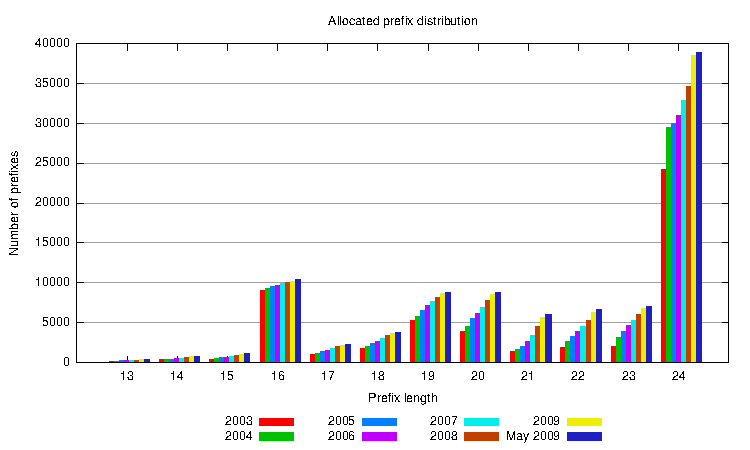
\includegraphics[width=0.5\textwidth]{02_prefixes/02_ip_prefixes_zoom}
	\caption{Allocated prefix distribution}
 	\label{fig:IP allocations}
\end{figure}

\subsection{Yearly distribution of IP allocations}

% \begin{figure}[htbp]
%  	\centering
%  		 \includegraphics[width=0.5\textwidth]{04_plus_minus/addremoveprefixallocculmulative}
% 	\caption{Trends in IP prefix allocation}
%  	\label{fig:IP allocations new and gone}
% \end{figure}

Aggregated together, the number of new allocations over the time period
studied is over 40,000. Figure \ref{fig:IP allocations new and gone} charts
the occurrence of other events that factor into the net allocation count
increase. These include prefix splitting, prefix extension, and deallocation.
Prefix splitting is the dividing of one prefix into multiple smaller prefixes.
Prefix extension is the aggregating of an existing prefix with its adjacent,
previously unallocated address space (e.g. a /16 prefix might become a /15
prefix by including the adjacent /16 address space). Deallocation is the
withdrawing of a prefix allocation, essentially releasing IP space for later
use. Figure \ref{fig:IP allocations new and gone}, charts these factors that
increase the count of allocations. Some of the increase is attributable to new
allocations. A smaller amount was due to prefix splitting. A small decrease in
the allocations count resulted from prefix extension. Finally, a larger
decrease was due to deallocation, although the number of new allocations has
greatly outpaced the disappearances.

\begin{figure}[htbp]
    \centering
        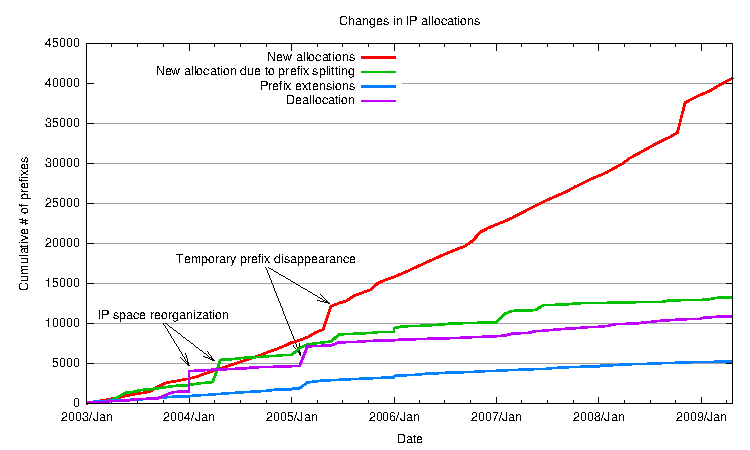
\includegraphics[width=\columnwidth]{04_3_plus_minus/changes}
    \caption{Changes in IP allocations}
    \label{fig:IP allocations new and gone}
\end{figure}

There is one illustration that particularly shows the dynamic character of IP
allocation records. Figure \ref{fig:alloc ages total} plots the number of
prefixes allocated each year, according to snapshots taken in the years from
2003 to 2009 (shown in different colors). It is interesting to note that in
more recent years, the record of prefixes allocated during the 1990s has
increased. This increase is especially prominent in the past year. Among other
reasons, this is indicative of prefix splitting, where a larger allocated
block is split into multiple blocks. When blocks are split, the resulting
blocks retain the year of origin of the block under which they were originally
allocated. Figure \ref{fig:alloc ages total} shows that while many of the
existing allocations originated in the 90s, many of these also are blocks
split off larger ones that were allocated at the time.

\begin{figure}[htbp]
	\centering
		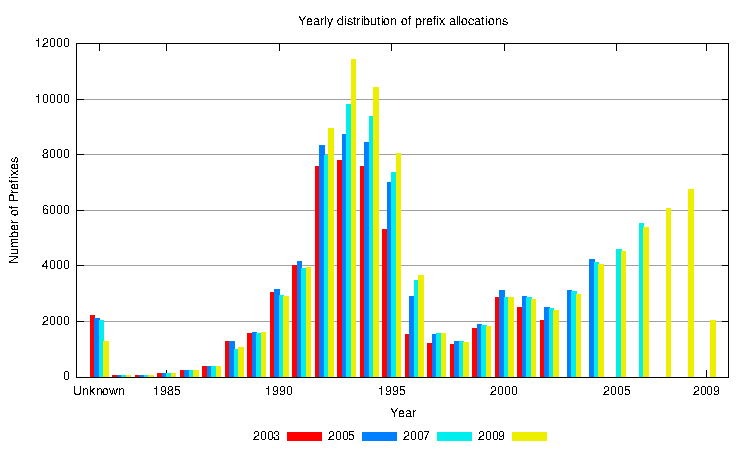
\includegraphics[width=\columnwidth]{10_alloc_ages/alloc_total}
	\caption{Records of IP allocations, from the perspective the given years
		     2003--2009 (odd-numbered years shown only, for clarity)}
	% \newline
	% * Note that in successive years, the known number of allocations recorded tends
	% to rise (odd-numbered years shown only, for clarity)}
	\label{fig:alloc ages total}
\end{figure}


\subsection{Unaligned allocation}

There is an occurrence among IP allocations that--while rare--warrants some
attention. Unaligned IP blocks are any allocations of a size that is not some
power of 2. For instance, an unaligned block of 12,288 addresses has been
recently allocated by ARIN (allocation of the block 67.23.0.0-67.23.47.255 on
January 23, 2009). This allocation cannot be represented as a single entry in
the BGP routing table and requires at least a /19 and /20 prefix to express it.
The number of unaligned allocations is very small because they clearly are
wasteful of BGP table space and have insignificant advantages over aligned
ones, if any. Figure~\ref{fig:unaligned IP allocations} shows the distribution
of such allocations. Most were between 1992 and 1995, although a few continue
to be allocated every year since then. Obviously, compared to the size of the
routing table ($>$300K entries) these allocations are negligible in number.
Nonetheless it is interesting to note their continued existence.

\begin{figure}[htbp]
 	\centering
 		\includegraphics[width=0.5\textwidth]{09_alloc_adhoc/adhoc}
	\caption{Unaligned IP allocations per year}
 	\label{fig:unaligned IP allocations}
\end{figure}

\subsection{Allocation by geographical region}

\begin{table*}[p]
%%%%%%%%%%%%%%%%%%%%%%%%%%%%%%%%%%%%%%%%%%%%%%%%%%%%%%%%%%%%%%%%%%%%%%%%%%%%%%%%
%% TOP announced prefixes
%%%%%%%%%%%%%%%%%%%%%%%%%%%%%%%%%%%%%%%%%%%%%%%%%%%%%%%%%%%%%%%%%%%%%%%%%%%%%%%%
\begin{minipage}[t]{0.48\textwidth}
% \begin{table}[p]
	\begin{center}
	\caption{Top 25 countries with the most number of allocated IP blocks on \textbf{January 1, 2003}}
	\label{tab:top25 rir prefixes 2003}
	\begin{tabular}{|l||l|r|r|}
		\hline
		&      \bf Country		& \bf Prefixes  &  \bf  IP space 		\tabularnewline \hline
1       &       US      		&       31,699  &       1,240,486,995   \tabularnewline
2       &       Canada  		&       5,314   &       61,593,600      \tabularnewline
3       &       Germany 		&       1,642   &       49,413,120      \tabularnewline
4       &       UK      		&       1,573   &       74,358,784      \tabularnewline
5       &       Australia       &       1,351   &       22,956,032      \tabularnewline
6       &       Italy   		&       836     &       14,270,464      \tabularnewline
7       &       Switzerland     &       737     &       10,523,904      \tabularnewline
8       &       Japan   		&       674     &       95,166,320      \tabularnewline
9       &       France  		&       625     &       37,038,080      \tabularnewline
10      &       Netherlands     &       619     &       28,387,328      \tabularnewline
11      &       Sweden  		&       533     &       13,377,024      \tabularnewline
12      &       Russia  		&       501     &       6,259,200       \tabularnewline
13      &       Hong Kong       &       491     &       4,476,416       \tabularnewline
14      &       China   		&       393     &       29,396,736      \tabularnewline
15      &       New Zealand     &       366     &       3,820,288       \tabularnewline
16      &       Finland 		&       348     &       8,085,760       \tabularnewline
17      &       Norway  		&       322     &       8,610,304       \tabularnewline
18      &       Spain   		&       310     &       9,625,344       \tabularnewline
19      &       South Africa    &       275     &       8,163,328       \tabularnewline
20      &       Austria 		&       267     &       5,279,232       \tabularnewline
21      &       Brazil  		&       260     &       10,902,784      \tabularnewline
22      &       Chile   		&       251     &       2,310,656       \tabularnewline
23      &       Singapore       &       250     &       1,933,856       \tabularnewline
24      &       Thailand        &       245     &       1,667,328       \tabularnewline
25      &       India   		&       240     &       2,636,032       \tabularnewline
% 26      &       South Korea     &       197     &       26,208,768      \tabularnewline
% 27      &       Indonesia       &       188     &       1,005,568       \tabularnewline
% 28      &       Taiwan  		&       184     &       11,659,008      \tabularnewline
% 29      &       Poland  		&       174     &       3,982,080       \tabularnewline
% 30      &       Belgium 		&       163     &       4,664,832       \tabularnewline
	\hline
	\end{tabular}
	\end{center}
% \end{table}
\end{minipage}
%
\quad
%
\begin{minipage}[t]{0.48\textwidth}
% \begin{table}[p]
	\begin{center}
	\caption{Top 25 countries with the most number of allocated IP blocks on \textbf{April 23, 2009}}
	\label{tab:top25 rir prefixes 2009}
	\begin{tabular}{|l||l|r|r|r|}
		\hline
		&      \bf Country		& \bf Prefixes  &       \bf IP space 	& \bf Change$^{*}$ 	\tabularnewline \hline 
1       &       US      &       36,881  &       1,473,990,144   &         1.16  \tabularnewline
2       &       Australia       &       6,099   &       37,378,304      &         4.51  \tabularnewline
3       &       Canada  &       5,709   &       75,905,792      &         1.07  \tabularnewline
4       &       Germany &       5,612   &       85,205,400      &         3.42  \tabularnewline
5       &       European Union  &       5,074   &       114,168,224     &        46.98  \tabularnewline
6       &       UK      &       3,732   &       70,756,184      &         2.37  \tabularnewline
7       &       Russia  &       3,148   &       24,607,688      &         6.28  \tabularnewline
8       &       Japan   &       2,068   &       153,285,376     &         3.07  \tabularnewline
9       &       France  &       1,814   &       68,384,704      &         2.90  \tabularnewline
10      &       Ukraine &       1,769   &       5,516,480       &        19.88  \tabularnewline
11      &       Poland  &       1,602   &       13,869,704      &         9.21  \tabularnewline
12      &       China   &       1,566   &       191,643,392     &         3.98  \tabularnewline
13      &       Netherlands     &       1,449   &       21,291,560      &         2.34  \tabularnewline
14      &       Switzerland     &       1,359   &       8,249,320       &         1.84  \tabularnewline
15      &       New Zealand     &       1,217   &       6,116,096       &         3.33  \tabularnewline
16      &       Italy   &       955     &       32,206,272      &         1.14  \tabularnewline
17      &       South Africa    &       886     &       15,057,920      &         3.22  \tabularnewline
18      &       Sweden  &       862     &       18,986,400      &         1.62  \tabularnewline
19      &       Austria &       854     &       7,292,128       &         3.20  \tabularnewline
20      &       Romania &       769     &       8,643,328       &        21.36  \tabularnewline
21      &       Czech Republic  &       706     &       6,059,392       &         5.98  \tabularnewline
22      &       South Korea     &       700     &       72,193,792      &         3.55  \tabularnewline
23      &       Finland &       655     &       8,932,864       &         1.88  \tabularnewline
24      &       Hong Kong       &       651     &       8,208,128       &         1.33  \tabularnewline
25      &       India   &       611     &       18,290,432      &         2.55  \tabularnewline
% 26      &       Spain   &       530     &       21,794,976      &         1.71  \tabularnewline
% 27      &       Denmark &       491     &       9,289,824       &         3.43  \tabularnewline
% 28      &       Indonesia       &       482     &       7,263,488       &         2.56  \tabularnewline
% 29      &       Taiwan  &       422     &       24,680,704      &         2.29  \tabularnewline
% 30      &       Argentina       &       421     &       7,395,072       &         2.75  \tabularnewline
	\hline
	\end{tabular}
	\end{center}

	\small	$^{*}$ -- Relative change in number of allocated IP blocks from January 1, 2003 and April 23, 2009
% \end{table}
\end{minipage}

\vspace{1cm}

%%%%%%%%%%%%%%%%%%%%%%%%%%%%%%%%%%%%%%%%%%%%%%%%%%%%%%%%%%%%%%%%%%%%%%%%%%%%%%%%
%% TOP announced IP space
%%%%%%%%%%%%%%%%%%%%%%%%%%%%%%%%%%%%%%%%%%%%%%%%%%%%%%%%%%%%%%%%%%%%%%%%%%%%%%%%
\begin{minipage}[t]{0.48\textwidth}
% \begin{table}[p]
	\begin{center}
	\caption{Top 25 countries with the most allocated IP space on \textbf{January 1, 2003}}
	\label{tab:top25 rir ip space 2003}
	\begin{tabular}{|l||l|r|r|}
		\hline
		&      \bf Country		& \bf Prefixes  &  \bf IP space 		\tabularnewline \hline 
1       &       US      		&       31,699  &       1,240,486,995   \tabularnewline
2       &       Japan   		&       674     &       95,166,320      \tabularnewline
3       &       UK      		&       1,573   &       74,358,784      \tabularnewline
4       &       Canada  		&       5,314   &       61,593,600      \tabularnewline
5       &       Germany 		&       1,642   &       49,413,120      \tabularnewline
6       &       France  		&       625     &       37,038,080      \tabularnewline
7       &       China   		&       393     &       29,396,736      \tabularnewline
8       &       Netherlands     &       619     &       28,387,328      \tabularnewline
9       &       South Korea     &       197     &       26,208,768      \tabularnewline
10      &       Australia       &       1,351   &       22,956,032      \tabularnewline
11      &       Italy   		&       836     &       14,270,464      \tabularnewline
12      &       Sweden  		&       533     &       13,377,024      \tabularnewline
13      &       Taiwan  		&       184     &       11,659,008      \tabularnewline
14      &       Brazil  		&       260     &       10,902,784      \tabularnewline
15      &       Switzerland     &       737     &       10,523,904      \tabularnewline
16      &       Spain   		&       310     &       9,625,344       \tabularnewline
17      &       Norway  		&       322     &       8,610,304       \tabularnewline
18      &       South Africa    &       275     &       8,163,328       \tabularnewline
19      &       Finland 		&       348     &       8,085,760       \tabularnewline
20      &       Russia  		&       501     &       6,259,200       \tabularnewline
21      &       Mexico  		&       132     &       5,644,288       \tabularnewline
22      &       Austria 		&       267     &       5,279,232       \tabularnewline
23      &       Belgium 		&       163     &       4,664,832       \tabularnewline
24      &       Denmark 		&       143     &       4,634,624       \tabularnewline
25      &       Hong Kong       &       491     &       4,476,416       \tabularnewline
% 26      &       Poland  		&       174     &       3,982,080       \tabularnewline
% 27      &       New Zealand     &       366     &       3,820,288       \tabularnewline
% 28      &       European Union  &       108     &       3,149,824       \tabularnewline
% 29      &       India  			&       240     &       2,636,032       \tabularnewline
% 30      &       Israel 			&       81      &       2,579,712       \tabularnewline
	\hline
	\end{tabular}
	\end{center}
	\ \newline\ \newline
% \end{table}
\end{minipage}
%
\quad
%
\begin{minipage}[t]{0.48\textwidth}
% \begin{table}[p]
	\begin{center}
	\caption{Top 25 countries with the most allocated IP space on \textbf{April 23, 2009}}
	\label{tab:top25 rir ip space 2009}
	\begin{tabular}{|l||l|r|r|r|}
		\hline
		&      \bf Country		& \bf Prefixes  &       \bf IP space 	& \bf Change$^{*}$ 	\tabularnewline \hline 
1       &       US      &       36,881  &       1,473,990,144   &         1.19  \tabularnewline
2       &       China   &       1,566   &       191,643,392     &         6.52  \tabularnewline
3       &       Japan   &       2,068   &       153,285,376     &         1.61  \tabularnewline
4       &       European Union  &       5,074   &       114,168,224     &        36.25  \tabularnewline
5       &       Germany &       5,612   &       85,205,400      &         1.72  \tabularnewline
6       &       Canada  &       5,709   &       75,905,792      &         1.23  \tabularnewline
7       &       South Korea     &       700     &       72,193,792      &         2.75  \tabularnewline
8       &       UK      &       3,732   &       70,756,184      &          .95  \tabularnewline
9       &       France  &       1,814   &       68,384,704      &         1.85  \tabularnewline
10      &       Australia       &       6,099   &       37,378,304      &         1.63  \tabularnewline
11      &       Italy   &       955     &       32,206,272      &         2.26  \tabularnewline
12      &       Brazil  &       267     &       29,754,880      &         2.73  \tabularnewline
13      &       Taiwan  &       422     &       24,680,704      &         2.12  \tabularnewline
14      &       Russia  &       3,148   &       24,607,688      &         3.93  \tabularnewline
15      &       Spain   &       530     &       21,794,976      &         2.26  \tabularnewline
16      &       Mexico  &       156     &       21,503,232      &         3.81  \tabularnewline
17      &       Netherlands     &       1,449   &       21,291,560      &          .75  \tabularnewline
18      &       Sweden  &       862     &       18,986,400      &         1.42  \tabularnewline
19      &       India   &       611     &       18,290,432      &         6.94  \tabularnewline
20      &       South Africa    &       886     &       15,057,920      &         1.84  \tabularnewline
21      &       Poland  &       1,602   &       13,869,704      &         3.48  \tabularnewline
22      &       Turkey  &       283     &       10,515,904      &         4.22  \tabularnewline
23      &       Denmark &       491     &       9,289,824       &         2.00  \tabularnewline
24      &       Finland &       655     &       8,932,864       &         1.10  \tabularnewline
25      &       Romania &       769     &       8,643,328       &        12.95  \tabularnewline
% 26      &       Switzerland     &       1,359   &       8,249,320       &          .78  \tabularnewline
% 27      &       Hong Kong       &       651     &       8,208,128       &         1.83  \tabularnewline
% 28      &       Norway  &       419     &       7,425,584       &          .86  \tabularnewline
% 29      &       Argentina       &       421     &       7,395,072       &         3.87  \tabularnewline
% 30      &       Austria &       854     &       7,292,128       &         1.38  \tabularnewline
	\hline
	\end{tabular}
	\end{center}
	\small	$^{*}$ -- Relative change in allocated IP space from January 1, 2003 and April 23, 2009
% \end{table}
\end{minipage}

\end{table*}

% \clearpage

\begin{figure*}[tp]
\begin{minipage}[b]{\textwidth}
\centering

%%%%%%%%%%%%%%%%%%%%%%%%%%%%%%%%%%%%%%%%%%%%%%%%%%%%%%%%%%%%%%%%%%
%% BGP counts
%%%%%%%%%%%%%%%%%%%%%%%%%%%%%%%%%%%%%%%%%%%%%%%%%%%%%%%%%%%%%%%%%%
\begin{minipage}[b]{0.48\textwidth}
% \begin{figure}[p]
	\centering
		\includegraphics[trim=0 17px 0px 76px,clip=true,width=\columnwidth]{00_maps/ip_count_2003}%
		\hspace{-0.98\columnwidth}%
		\includegraphics[width=1cm]{scale_ip_count}\hspace{-1cm}%
		\hspace{0.98\columnwidth}
	\caption{Geographical distribution of number of allocated IP blocks on \textbf{January 1, 2003}}
	\label{fig:rir prefixes 2003}
% \end{figure}
\end{minipage}%
%
\quad
%
\begin{minipage}[b]{0.48\textwidth}
% \begin{figure}[p]
	\centering
		\includegraphics[trim=0 17px 0px 76px,clip=true,width=\columnwidth]{00_maps/ip_count_2009_2}%
		\hspace{-0.98\columnwidth}%
		\includegraphics[width=1cm]{scale_ip_count}\hspace{-1cm}%
		\hspace{0.98\columnwidth}
	\caption{Geographical distribution of number of allocated IP blocks on \textbf{April 23, 2009}}
	\label{fig:rir prefixes 2009}
% \end{figure}
\end{minipage}

\vspace{0.5cm}

%%%%%%%%%%%%%%%%%%%%%%%%%%%%%%%%%%%%%%%%%%%%%%%%%%%%%%%%%%%%%%%%%%
%% BGP sizes
%%%%%%%%%%%%%%%%%%%%%%%%%%%%%%%%%%%%%%%%%%%%%%%%%%%%%%%%%%%%%%%%%%
\begin{minipage}[b]{0.48\textwidth}
% \begin{figure}[p]
	\centering
		\includegraphics[trim=0 17px 0px 76px,clip=true,width=\columnwidth]{00_maps/ip_size_2003}%
		\hspace{-0.98\columnwidth}%
		\includegraphics[width=1cm]{scale_ip_size}\hspace{-1cm}%
		\hspace{0.98\columnwidth}
	\caption{Geographical distribution of allocated IP space on \textbf{January 1, 2003}}
	\label{fig:rir ip space 2003}
% \end{figure}
\end{minipage}%
%
\quad
%
\begin{minipage}[b]{0.48\textwidth}
% \begin{figure}[p]
	\centering
		\includegraphics[trim=0 17px 0px 76px,clip=true,width=\columnwidth]{00_maps/ip_size_2009_2}%
		\hspace{-0.98\columnwidth}%
		\includegraphics[width=1cm]{scale_ip_size}\hspace{-1cm}%
		\hspace{0.98\columnwidth}
	\caption{Geographical distribution of allocated IP space on \textbf{April 23, 2009}}
	\label{fig:rir ip space 2009}
% \end{figure}
\end{minipage}

\vspace{0.5cm}

%%%%%%%%%%%%%%%%%%%%%%%%%%%%%%%%%%%%%%%%%%%%%%%%%%%%%%%%%%%%%%%%%%
%% Asia region
%%%%%%%%%%%%%%%%%%%%%%%%%%%%%%%%%%%%%%%%%%%%%%%%%%%%%%%%%%%%%%%%%%
\begin{minipage}[b]{0.48\textwidth}
% \begin{figure}[p]
	\centering
		\includegraphics[trim=0 17px 0px 76px,clip=true,width=\columnwidth]{00_maps/ip_asia_2009_prefixes}%
		\hspace{-0.98\columnwidth}%
		\includegraphics[width=1cm]{scale_ip_count}\hspace{-1cm}%
		\hspace{0.98\columnwidth}
	\caption{Geographical distribution of number of allocated IP blocks in Asian region on \textbf{April 23, 2009}}
	\label{fig:rir prefixes asia 2009}
% \end{figure}
\end{minipage}%
%
\quad
%
\begin{minipage}[b]{0.48\textwidth}
% \begin{figure}[p]
	\centering
		\includegraphics[trim=0 17px 0px 76px,clip=true,width=\columnwidth]{00_maps/ip_asia_2009_space}%
		\hspace{-0.98\columnwidth}%
		\includegraphics[width=1cm]{scale_ip_size}\hspace{-1cm}%
		\hspace{0.98\columnwidth}
	\caption{Geographical distribution of allocated IP space in Asian region on \textbf{April 23, 2009}}
	\label{fig:rir ip space asia 2009}
% \end{figure}
\end{minipage}

\end{minipage}
\end{figure*}

% \clearpage


In this part we present a number of findings of IP allocations from a 
geographical viewpoint, that is, on a country-based level. The analysis of 
snapshots of IP allocations at fixed times shows which countries are 
allocated more prefixes and gives an understanding of the Internet penetration 
throughout the world.

Table~\ref{tab:top25 rir prefixes 2003} is a list of the 25 countries that 
were allocated the most prefixes in 2003.  With each country is shown what 
size of IP address space is covered by the sets of allocated IP blocks.
Table~\ref{tab:top25 rir ip space 2003} gives an alternative representation, 
re-ordered by descending IP-allocated space.  We note that, for example, 
in 2003 Japan with only 674 allocated prefixes (8th in 
Table~\ref{tab:top25 rir prefixes 2003}) covered more IP (2nd in 
Table~\ref{tab:top25 rir ip space 2003}) space than all other countries 
excluding the United States.  This indicates Japan's allocations efficiently 
cover their IP space.

Tables~\ref{tab:top25 rir prefixes 2009} and ~\ref{tab:top25 rir ip space
2009} present a current estimates for 2009 of the same data, name the 
top 25 contributors to the global routing table and top 25 countries with 
the most announced address space. A comparison of the 2003 and 2009 tables 
shows a marked re-ordering of some countries relative to others, in terms 
of the number of allocations as well as in terms of the number of allocated 
IP addresses. For example, Canada (2nd in 
Table~\ref{tab:top25 rir prefixes 2003}) had relatively small growth over 
the 6 years and is now tied in rank with other regions that made great strides, 
such as Australia (5th in Table~\ref{tab:top25 rir prefixes 2003}, 
2nd in Table~\ref{tab:top25 rir prefixes 2009}) and the European countries 
(a combined entity recognized during the 6-year interval).

Figures~\ref{fig:rir prefixes 2003}--\ref{fig:rir ip space asia 2009} show the
annual number of allocations by colors on a map of the world\footnote{%
An extended number of interactive colored maps for years 2003--2004 are 
available in \url{http://map.iu4.ru}
}
%
. The figure pairs 
\ref{fig:rir prefixes 2003} \& \ref{fig:rir prefixes 2009}, and 
\ref{fig:rir ip space 2003} \& \ref{fig:rir ip space 2009}, trace regional Internet 
growth dynamics from a global view.  These world maps repeat the information given 
in Tables~\ref{tab:top25 rir prefixes 2003}--~\ref{tab:top25 rir ip space
2009} but also include relative allocation activity levels for all countries of 
the world.  Figure~\ref{fig:rir prefixes asia 2009} and 
Figure~\ref{fig:rir ip space asia 2009} reiterate the measure of IP space usage
``efficiency'' in one section of the world undergoing tremendous Internet penetration 
and growth.  In East Asia several countries such as Japan and China, using fewer allocated 
block (lighter colors in Figure ~\ref{fig:rir prefixes asia 2009}), 
cover much more IP space (darker colors in Figure~\ref{fig:rir ip space asia 2009}), 
in comparison to a country such as India.


\section{BGP routing table}
\label{sec:bgp}

In this section we present an evaluation of the global routing table from 2003
to 2009. We first analyze contributing causes to the growth of the global
routing table. This involves assessing a measure of how well ISPs tend to use
an allocated address space and how allocated address blocks are subdivided. The
second point of interest is to analyze the contents of the BGP routing table
itself. This includes determining the extent that IP prefix announcements
overlap (i.e., how many individual prefixes are also parts of bigger prefixes
present in the same routing table). We also discuss a measure of the stability
of the routing table contents. For this measurement, we calculate the time
period during which an individual prefix was visible to the BGP monitor.
Finally, in an analogous fashion to the previous section, we present an
analysis of the BGP routing table dynamics grouped by the geographical region.
We conclude with identifying countries with the largest number of announced
prefixes.

%%%%%%%%%%%%%%%%%%%%%%%%%%%%%%%%%%%%%%%%%%%%%%%%%%%%%%%%%%%%%%%%%%%%%%%%%%%%%
%%%%%%%%%%%%%%%%%%%%%%%%%%%%%%%%%%%%%%%%%%%%%%%%%%%%%%%%%%%%%%%%%%%%%%%%%%%%%
%%%%%%%%%%%%%%%%%%%%%%%%%%%%%%%%%%%%%%%%%%%%%%%%%%%%%%%%%%%%%%%%%%%%%%%%%%%%%
\subsection{Analysis of BGP table growth factors}
%%%%%%%%%%%%%%%%%%%%%%%%%%%%%%%%%%%%%%%%%%%%%%%%%%%%%%%%%%%%%%%%%%%%%%%%%%%%%
%%%%%%%%%%%%%%%%%%%%%%%%%%%%%%%%%%%%%%%%%%%%%%%%%%%%%%%%%%%%%%%%%%%%%%%%%%%%%
%%%%%%%%%%%%%%%%%%%%%%%%%%%%%%%%%%%%%%%%%%%%%%%%%%%%%%%%%%%%%%%%%%%%%%%%%%%%%

The BGP routing table is growing at a rate significantly higher than the pace
that RIRs are allocating IP blocks. Across all BGP monitors we observed, the
average number of entries in the global routing table is more than 3 times the
number of IP blocks that RIRs have allocated (refer Figure~\ref{fig:BGP vs
RIR}). This multiplication in size reflects two primary practices. First, ISPs
tend to subdivide allocated IP blocks into several individual prefixes and
announce them separately. Such behavior is typical, for example, among
transnational providers as well as among ISP customers that have been lent
parts of their service providers' address space and in turn independently
announce subdivided IP address blocks. Second, various traffic engineering
techniques (traffic balancing, multihoming, etc.) give rise to situations where
the same address block is covered by several announced prefixes.

\subsubsection{IP block fragmentation}

The contents of the BGP routing table consist of IP prefixes that either match,
fragment, or aggregate various IP allocation blocks.
Figure~\ref{fig:fragmentation} shows the correlation between allocated IP
blocks and announced IP prefixes and the relative proportions of these three
categories over time. The \emph{matched} curve in the figure represents IP
blocks that are announced in the routing table in the exact form as they were
issued by RIRs. An example of a matched prefix announcement is an appearance in
the table of a /22 prefix (equivalent to 1,024 IP addresses) that was issued in
just that form by an ISP. As is evident in the figure, the number of matched
prefixes accounts for 1/6 the total number of BGP entries at the present time,
with the trend that this fraction is growing smaller over time.

\begin{figure}[htbp]
	\centering
		\includegraphics[width=\columnwidth]{05_matched_fragmented/frag-3}
	\caption{Dynamics of matched, fragmented, and aggregated IP prefixes in BGP announcements}
	\label{fig:fragmentation}
\end{figure}

ISPs are evidently not inclined to distribute address space often in the form
in which it was allocated. For various possible reasons (e.g., geographical
dispersion), ISPs split up allocated blocks into a number of sub-blocks and
announce each of these independently. The \emph{fragmented} curve in
Figure~\ref{fig:fragmentation} represents these subdivided blocks, which
account for more than 83\% of all entries in the global routing table. IP block
fragmentation poses one of the primary concerns for future scalability of the
BGP routing table.

The lowest curve, \emph{aggregated}, represents IP prefix announcements that
cover several allocated IP blocks. For these cases---in contrast to
fragmentation---ISPs that have several adjacent IP block allocations simply
announce them as a single IP prefix. As the figure illustrates, this
aggregation technique is rarely employed to any measure. Its primary intent, to
reduce the number of entries in the routing table, is outweighed for more often
by other policy routing choices. The number of aggregated prefixes in 2003 was
1,400. By 2009 this number increased only marginally, to just under 2,000
prefixes, accounting for under 1\% of the entire routing table and reasonably
considered negligible in impact.

This observed behavior has a measure of relevance to future IPv6 deployment.
ISPs tend not to announce their allocated IP spaces in their original form.
Significantly, this behavior occurs regardless of the size of IP block that an
ISP was allocated. With regard to IPv6 deployment, the significance of this
point is as follows. According to current RIR policy, the minimum allocation
for an IPv6 block is /32 \cite{APNIC:2009:IPv6-Address}. In terms of expense,
the price of an IPv6 /32 block is the same as for a /19 or /20 IPv4 address
block \cite{ARIN:2009:Annual-Fee-Scedule}, meaning for an equivalent cost of
obtaining under 10,000 IPv4 prefixes, ISPs can be assigned an IPv6 block of a
size several orders of magnitude larger than the entire IPv4 space at present.
If allocations of large blocks continue, it is likely to mitigate the problem
of multiple, non-adjacent IP block allocations per customer. However, without a
major change in the BGP protocol aimed at lessening incentives to announce
fragmented IP prefixes, increasing the size of the IP block will not
significantly assist in reducing the size of global routing table. Table size
reduction stems only from aggregatable and matching IP prefixes. In other
words, only ISPs that currently use all allocated IP space as a single IP block
(i.e., matched or aggregated) would have any likelihood of using a bigger space
provided in IPv6 also as a single block. We conclude that the upper bound of IP
space announcement optimization is limited by the number of matched prefixes,
which currently stands at less than 17\% of all prefixes.

\subsubsection{Duplicate announcements of IP blocks}

The BGP routing table has a consistent pattern of containing a large number of
prefix ranges that duplicate each other (Figure~\ref{fig:covered}). IP address
coverage duplication assists calculating an actual route by matching the
destination address with the longest available prefix.  Address duplication in
a routing table is, in theory, an effective way to reduce the size of the
routing table itself. The following example illustrates this point: If we
consider an ISP that owns a /8 address block and that wants a particular /24
block routed in a special way, using a different path than the rest of the
block, it is much more effective to use a small duplication of address space
and only two entries in the routing table (the /8 and the /24 prefixes) than
avoiding duplication and announcing 65,536 individual /24 prefixes.

\begin{figure}[htbp]
	\centering
		\includegraphics[width=\columnwidth]{06_covered/cover-3}
	\caption{Relative numbers of \emph{covered}, \emph{covering}, and \emph{unique} IP prefixes among BGP announcements}
	\label{fig:covered}
\end{figure}

Our observations indicate that ISPs extensively use the fundamental IP routing
feature of longest-prefix matching. As Figure~\ref{fig:covered} shows by the
\emph{1-level} and \emph{unique} curves, the number of IP prefixes in BGP table
which are covered by exactly one bigger prefix is nearly the same as the number
of unique prefixes (i.e., base prefixes). There is moreover a substantial
number of prefixes that have several layers of coverage (several duplication
levels---refer to \emph{2+-level} curve).

These high proportions of 1-level and 2+-level covered prefixes indicate there
are other incentives and benefits for prefix duplication, in addition to the
theoretical routing table optimization. One factor we consider is a
multi-provider connection for end-networks (so-called multihoming of \emph{stub
networks}). According to Oliveira et al.
\cite{Oliveira:2007:Observing-the-evolution}, more than 70\% of all
announcements belong to multihomed stub networks. In other words, the global
routing table was adopted to serve local or semi-local routing interests for
most customers. Since these routing interests extend out on a primarily local
scale, it would seem unlikely that the outside world would follow widely
divergent routing paths to reach various providers' connections to a multihomed
customer (a stub network). Thus while the need for covered prefixes is evident
to accommodate these routing preferences, they need not be shared universally
in routing tables. We conclude that to significantly reduce the size of the BGP
routing table, there should be counter-incentives to IP prefix fragmentation.
As an area of further research, for example, separate means for multihoming and
traffic engineering tasks might be provided.

%%%%%%%%%%%%%%%%%%%%%%%%%%%%%%%%%%%%%%%%%%%%%%%%%%%%%%%%%%%%%%%%%%%%%%%%%%%%%
%%%%%%%%%%%%%%%%%%%%%%%%%%%%%%%%%%%%%%%%%%%%%%%%%%%%%%%%%%%%%%%%%%%%%%%%%%%%%
%%%%%%%%%%%%%%%%%%%%%%%%%%%%%%%%%%%%%%%%%%%%%%%%%%%%%%%%%%%%%%%%%%%%%%%%%%%%%
\subsection{Analysis of the BGP table contents}
%%%%%%%%%%%%%%%%%%%%%%%%%%%%%%%%%%%%%%%%%%%%%%%%%%%%%%%%%%%%%%%%%%%%%%%%%%%%%
%%%%%%%%%%%%%%%%%%%%%%%%%%%%%%%%%%%%%%%%%%%%%%%%%%%%%%%%%%%%%%%%%%%%%%%%%%%%%
%%%%%%%%%%%%%%%%%%%%%%%%%%%%%%%%%%%%%%%%%%%%%%%%%%%%%%%%%%%%%%%%%%%%%%%%%%%%%

In this part we examine the contents that comprise the BGP routing table. By
analyzing changes in its contents over the period from 2003 to 2009 we can
deduce current trends and demands for the IP space. Later in this part, we
share the distribution of prefix sizes announced in the table, the lifespan
(longevity) of IP prefix announcements, and the distribution of the IP space
from a geographical standpoint.

\subsubsection{Lengths of announced IP prefixes}

Critical questions in the global routing system are the following: (1) What is
an optimal length of IP prefix to allocate to customers? and (2) What is the
optimal algorithm to select a right prefix to allocate (in other words, how
much space should RIRs or ISPs reserve after an allocated block to accommodate
repeated requests from the same customer, and still maintain the customer's
allocations adjacent to each another, reducing fragmentation)? A number of
solutions propose to resolve the latter question, including sequential and
bisection allocation schemes and the GAP algorithm
\cite{Wang:2007:Reduce-IP-Address}. The former is still an open research
question.

To explore an answer to the first question, we present current statistics of
prefix lengths that have appeared in the routing table since 2003.
 Figure~\ref{fig:bgp prefix distribution} presents the distribution of
announced prefix lengths, classified by each year. The majority of the global
routing table entries are /24-length prefixes and account for more than 53\% of
entries. Among statistics for /24 prefixes, it is notable that the number of
/24 prefixes has nearly doubled between 2003 and 2009. At the same time, the
number of allocated blocks actually /24 in size is 4 times smaller (refer
Figure~\ref{fig:IP allocations}). This again gives evidence that a large number
of stub networks (i.e., relatively small customer networks) use announcements
of small address blocks to implement multi-provider connectivity.

\begin{figure}[htbp]
	\centering
		\includegraphics[width=\columnwidth]{02_prefixes/01_bgp_prefixes_zoom}
	\caption{Distribution of announced IP prefix lengths}
	\label{fig:bgp prefix distribution}
\end{figure}

Several other observations can be made from Figure~\ref{fig:bgp prefix
distribution}. Prefix lengths of /16--/23 (in comparison to /24 lengths) have
relatively the same level of popularity in the global routing table, among
which /17 and /18 constitute the least popular. The most dynamic prefixes among
this group over the 6 years are /20 and /21 (2.8 and 3.7 times growth,
respectively), and the least dynamic is /16 (1.4 times growth). Another
interesting observation concerns /16 prefixes. From among the most numerous
kinds of prefix lengths announced in the routing table (/16--/24), only the
number of /16 prefixes announced in the routing table closely matches the
number of allocations (again refer Figure~\ref{fig:IP allocations}). All the
other most popular prefix lengths comprising the routing table have markedly
higher counts of announced prefixes in the table than were originally
allocated, giving further indication of prevalent fragmentation.

The rest of the prefixes (shorter than /16, longer than /24) have a marginal
presence in the global routing table.  Together, they number less than 8,000
prefixes ($<$3\%). This fact testifies to a small number of entities having large
(/8--/15) prefixes, and a small number of a tiny customer networks (prefixes
/25--/32) with a multi-provider connectivity.

The results in this section are additional evidence of the tight relationship
between global routing table growth and IP space fragmentation and duplication.
If we could suppress the majority of non-global related (i.e., locally
concerned) announcements, such as bursts of /24 prefixes due to local traffic
engineering, local and semi-local multihoming support, etc., the size of the
global routing table would be significantly reduced.

\subsubsection{Longevity distribution of BGP entries}

Another aspect of the BGP announcement analysis is determining the stability of
the global routing table. The distribution of prefix longevity is shown in
Figure~\ref{fig:bgp ages}. The bar on the far right of the graph indicates that
more than 15\% of the global routing table never changes over the course of our
period of study. On the other, far-left side, approximately another 15\% of the
prefixes
% (if we compare to the global routing table size in 2009)
 are active for only a short period of time. A small part of these
short-lived prefixes is likely comprised of spammers, who are known to hijack
someone's (or nobody's) prefix, announce it for a brief time, and send
virtually untraceable spam messages
\cite{Ramachandran:2006:Understanding-the-network-level}. Another portion of
short-lived prefixes can be attributed to configuration errors. The rest can be
explained by normal BGP operations, where some prefix becomes visible briefly
in such circumstances as when a primary network channel malfunctions.

\begin{figure}[htbp]
	\centering
		\includegraphics[width=\columnwidth]{08_ages/ages-4}
	\caption{Longevity of prefixes in BGP announcements}
	\label{fig:bgp ages}
\end{figure}

Excluding the unchanging portion of the BGP table contents shown in
Figure~\ref{fig:bgp ages}, the prefix longevity distribution follows to some
extent the exponential distribution function. In other words, announced
prefixes are likely to have a small longevity.  Besides a fixed number of
highly stable routes (15\%), the tapering-off shape of the distribution
suggests it is unlikely that a given route is visible for very long time. This
observation underscores that the composition of the routing table is highly
dynamic.

\subsubsection{BGP announcements by geographical region}

Finally, in examining the global routing table content, we present a
country-based analysis of the distribution of globally announced IP prefixes.
As with the allocation data, fixed-time snapshots point out the major
contributors to the global routing table and give an understanding of the
Internet's penetration throughout the world.

Table~\ref{tab:top25 bgp prefixes 2003} lists the top 25 contributors to the
global routing table in 2003 and gives the corresponding actual IP address
space that the announced prefixes cover. Table~\ref{tab:top25 bgp ip space
2003} gives an alternative representation for the BGP data snapshot from 2003,
where countries are listed in descending order by the number of IP addresses
covered by BGP announcements. To achieve these results, we matched announced
address spaces with corresponding allocated address spaces.  Due to the limited
nature of our IP prefix country association technique, there is a considerable
portion of the prefixes for which it was not possible to establish such an
association. Globally announced prefixes with undetermined ownership (shown as
\emph{Unknown}) in fact constitute the second largest contributor to the
routing table in 2003, after the United States. Holding third and fourth place
in 2003 were Australia and Canada. It should be mentioned that geographical
distributions, both of announced IP prefixes (Figure~\ref{fig:prefix distr})
and of announced IP space (Figure~\ref{fig:size distr}), have a stable,
quasi-exponential tapering shape.  The plot lines in both cases show minimal
variation in shape of the plot between 2003 and 2009.

\begin{figure}[htbp]
	\centering
		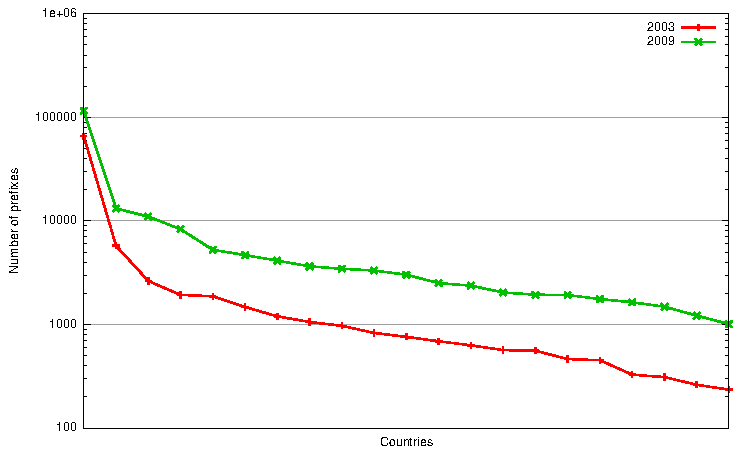
\includegraphics[width=\columnwidth]{01_bgp_ip_size/prefix-distr}
	\caption{Geographical distribution of globally announced IP prefixes (log scale)}
	\label{fig:prefix distr}
\end{figure}

\begin{figure}[htbp]
	\centering
		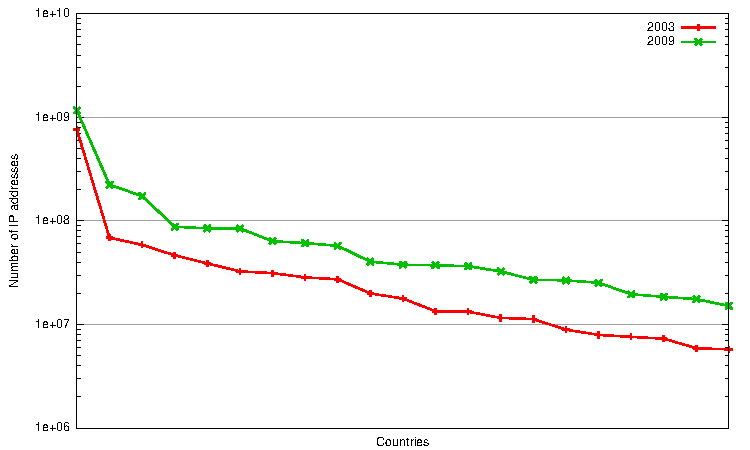
\includegraphics[width=\columnwidth]{01_bgp_ip_size/size-distr}
	\caption{Geographical distribution of globally announced IP space (log scale)}
	\label{fig:size distr}
\end{figure}

Tables~\ref{tab:top25 bgp prefixes 2009} and ~\ref{tab:top25 bgp ip space 2009}
present estimates for 2009 of the top 25 contributors to the global routing
table and the top 25 countries with the most announced address space. Again,
matched side-by-side with their 2003 counterparts, they provide easy comparison
of changes over time.  All countries contribute in greater numbers to the BGP
table. At the same time, the number of prefixes with undetermined ownership
(and the corresponding IP space) diminishes substantially by about half. The
United States retains its leading position. Meanwhile the ordering of the rest
contributors has significantly changed. South Korea has become the second major
contributor to the size of the global routing table, and China, Australia, and
India (having roughly the same number of announcements) rank third.

In terms of IP space usage, China, Japan, the European Union, Germany, and
South Korea are responsible over the most amount of announced address space
behind the United States. These four countries are a different ordering from
the number of announcements attributed in the routing table to a given country
(Table~\ref{tab:top25 bgp prefixes 2009}). This fact highlights that some
countries announce a large number of relatively small prefixes (e.g., in South
Korea one prefix on average covers 5,900 addresses), and some announce a small
number of large prefixes (e.g., in Japan one prefix covers on average 37,200
addresses). If this difference in usage efficiency occurs because of additional
government regulations, then for future IPv6 deployment, a similar host of
regulations should be considered globally.

 % are extremely efficient from BGP point of view

An alternative way to represent each country's contribution to the global
routing table is through color-coded diagrams in Figures~\ref{fig:bgp prefixes
2003}--\ref{fig:bgp ip space asia 2009}.%
%
\footnote{%
An extended number of interactive colored maps for years 2003--2009 are
available at \url{http://maps.iu4.ru}}%
%
 The figure pairs~\ref{fig:bgp prefixes 2003} \&~\ref{fig:bgp prefixes 2009},
as well as~\ref{fig:bgp ip space 2003} \&~\ref{fig:bgp ip space 2009}, make it
possible to trace the regional Internet growth dynamics. Figures~\ref{fig:bgp
prefixes asia 2009} and~\ref{fig:bgp ip space asia 2009} emphasize once again
differences of the varying effectiveness of IP space utilization (e.g., Japan
has many more addresses per announced prefix than compared to India or South
Korea).


\begin{table*}[tp]
%%%%%%%%%%%%%%%%%%%%%%%%%%%%%%%%%%%%%%%%%%%%%%%%%%%%%%%%%%%%%%%%%%%%%%%%%%%%%%%%
%% TOP announced prefixes
%%%%%%%%%%%%%%%%%%%%%%%%%%%%%%%%%%%%%%%%%%%%%%%%%%%%%%%%%%%%%%%%%%%%%%%%%%%%%%%%
\begin{minipage}[t]{0.48\textwidth}
% \begin{table}[p]
	\begin{center}
	\caption{Top 25 countries with the most number of announced prefixes in BGP table on \textbf{January 1, 2003}}
	\label{tab:top25 bgp prefixes 2003}
	\begin{tabular}{|l||l|r|r|} %\hline
		\hline
		&      \bf Country		&    Prefixes   &       IP space 		\tabularnewline \hline 
1       &       US      		&       65849   &       759,792,816     \tabularnewline %\hline
2       &       \emph{Unknown}	&       6258    &       68,926,314      \tabularnewline %\hline
3       &       Australia       &       5762    &       17,822,159      \tabularnewline %\hline
4       &       Canada  		&       5612    &       38,912,924      \tabularnewline %\hline
5       &       Japan   		&       2633    &       58,905,280      \tabularnewline %\hline
6       &       South Korea     &       2441    &       27,334,687      \tabularnewline %\hline
7       &       Germany			&       1934    &       46,556,556      \tabularnewline %\hline
8       &       India  			&       1931    &       2,943,040       \tabularnewline %\hline
9       &       UK     			&       1873    &       32,626,649      \tabularnewline %\hline
10      &       China  			&       1615    &       28,522,130      \tabularnewline %\hline
11      &       Argentina       &       1477    &       2,017,448       \tabularnewline %\hline
12      &       Hong Kong       &       1261    &       5,621,473       \tabularnewline %\hline
13      &       Sweden  		&       1198    &       11,280,533      \tabularnewline %\hline
14      &       France  		&       1148    &       31,320,040      \tabularnewline %\hline
15      &       Mexico  		&       1059    &       5,275,520       \tabularnewline %\hline
16      &       Romania 		&       994     &       667,136 		\tabularnewline %\hline
17      &       Russia  		&       972     &       5,911,712       \tabularnewline %\hline
18      &       Chile   		&       834     &       2,098,161       \tabularnewline %\hline
19      &       Indonesia       &       830     &       1,170,560       \tabularnewline %\hline
20      &       Italy   		&       791     &       13,324,288      \tabularnewline %\hline
21      &       Brazil  		&       760     &       11,580,416      \tabularnewline %\hline
22      &       Taiwan  		&       708     &       13,448,168      \tabularnewline %\hline
23      &       Netherlands     &       689     &       19,939,341      \tabularnewline %\hline
24      &       European Union  &       687     &       2,707,383       \tabularnewline %\hline
25      &       Finland 		&       630     &       7,307,018       \tabularnewline %\hline
% 26      &       South Africa    &       618     &       5,762,180       \tabularnewline %\hline
% 27      &       New Zealand     &       566     &       3,828,620       \tabularnewline %\hline
% 28      &       Switzerland     &       560     &       7,937,424       \tabularnewline %\hline
% 29      &       Thailand        &       559     &       1,877,060       \tabularnewline %\hline
% 30      &       Spain   		&       511     &       8,921,568       \tabularnewline %\hline
	\hline
	\end{tabular}
	\end{center}
% \end{table}
\end{minipage}
%
\quad
%
\begin{minipage}[t]{0.48\textwidth}
% \begin{table}[p]
	\begin{center}
	\caption{Top 25 countries with the most number of announced prefixes in BGP table on \textbf{April 23, 2009}}
	\label{tab:top25 bgp prefixes 2009}
	\begin{tabular}{|l||l|r|r|r|}
		\hline
		&      \bf Country		& \bf Prefixes  &       \bf IP space 	& \bf Change$^{*}$ 	\tabularnewline \hline 
1       &       US      		&       115780  &       1,170,481,177   & 1.54			\tabularnewline %\hline
2       &       South Korea     &       14308   &       84,553,300      & 3.09			\tabularnewline %\hline
3       &       China  			&       13188   &       223,990,021     & 7.85			\tabularnewline %\hline
4       &       Australia       &       11329   &       37,818,072      & 2.12			\tabularnewline %\hline
5       &       India   		&       11022   &       17,575,040      & 5.97			\tabularnewline %\hline
6       &       Russia  		&       8650    &       26,664,224      & 4.51			\tabularnewline %\hline
7       &       Canada  		&       8328    &       57,471,348      & 1.48			\tabularnewline %\hline
8       &       Romania 		&       5729    &       7,348,881       & 11.02			\tabularnewline %\hline
9       &       UK      		&       5269    &       63,871,082      & 1.96			\tabularnewline %\hline
10      &       European Union  &       4937    &       87,825,582      & 32.44			\tabularnewline %\hline
11      &       Japan   		&       4674    &       173,789,965     & 2.95			\tabularnewline %\hline
12      &       Brazil  		&       4643    &       40,429,504      & 3.49			\tabularnewline %\hline
13      &       Argentina       &       4142    &       9,721,411       & 4.82			\tabularnewline %\hline
14      &       Germany 		&       4035    &       84,904,642      & 1.82			\tabularnewline %\hline
15      &       Mexico  		&       3648    &       19,583,832      & 3.71			\tabularnewline %\hline
16      &       Indonesia       &       3562    &       5,248,256       & 4.48			\tabularnewline %\hline
17      &       Hong Kong       &       3459    &       14,764,300      & 2.63			\tabularnewline %\hline
18      &       \emph{Unknown}	&       3393    &       37,265,411      & 				\tabularnewline %\hline
19      &       Bulgaria        &       3325    &       4,439,040       & 7.72			\tabularnewline %\hline
20      &       Colombia        &       3029    &       4,901,340       & 11.86			\tabularnewline %\hline
21      &       Ukraine 		&       3028    &       5,547,136       & 7.67			\tabularnewline %\hline
22      &       Egypt  			&       2992    &       3,854,848       & 4.60			\tabularnewline %\hline
23      &       France 			&       2511    &       61,070,996      & 1.95			\tabularnewline %\hline
24      &       Taiwan 			&       2511    &       36,623,744      & 2.72			\tabularnewline %\hline
25      &       Chile  			&       2375    &       6,101,376       & 2.91			\tabularnewline %\hline
% 26      &       Poland 			&       2341    &       15,122,881      & 4.06			\tabularnewline %\hline
% 27      &       Thailand        &       2039    &       7,210,800       & 3.84			\tabularnewline %\hline
% 28      &       Spain   		&       1989    &       25,315,136      & 2.84			\tabularnewline %\hline
% 29      &       Sweden  		&       1942    &       18,532,345      & 1.64			\tabularnewline %\hline
% 30      &       Turkey  		&       1940    &       14,309,632      & 6.41			\tabularnewline %\hline
	\hline
	\end{tabular}
	\end{center}
	
	\small	$^{*}$ -- Relative change in number of prefixes in BGP announcements from January 1, 2003 and April 23, 2009
% \end{table}
\end{minipage}

\vspace{1cm}

%%%%%%%%%%%%%%%%%%%%%%%%%%%%%%%%%%%%%%%%%%%%%%%%%%%%%%%%%%%%%%%%%%%%%%%%%%%%%%%%
%% TOP announced IP space
%%%%%%%%%%%%%%%%%%%%%%%%%%%%%%%%%%%%%%%%%%%%%%%%%%%%%%%%%%%%%%%%%%%%%%%%%%%%%%%%
\begin{minipage}[t]{0.48\textwidth}
% \begin{table}[p]
	\begin{center}
	\caption{Top 25 countries with the most number of announced IP space in BGP table on \textbf{January 1, 2003}}
	\label{tab:top25 bgp ip space 2003}
	\begin{tabular}{|l||l|r|r|}
		\hline
		&      \bf Country		&    Prefixes   &       IP space 		\tabularnewline \hline 
1       &       US      		&       65849   &       759,792,816     \tabularnewline %\hline
2       &       \emph{Unknown} 	&       6258    &       68,926,314      \tabularnewline %\hline
3       &       Japan   		&       2633    &       58,905,280      \tabularnewline %\hline
4       &       Germany 		&       1934    &       46,556,556      \tabularnewline %\hline
5       &       Canada  		&       5612    &       38,912,924      \tabularnewline %\hline
6       &       UK      		&       1873    &       32,626,649      \tabularnewline %\hline
7       &       France  		&       1148    &       31,320,040      \tabularnewline %\hline
8       &       China   		&       1615    &       28,522,130      \tabularnewline %\hline
9       &       South Korea     &       2441    &       27,334,687      \tabularnewline %\hline
10      &       Netherlands     &       689     &       19,939,341      \tabularnewline %\hline
11      &       Australia       &       5762    &       17,822,159      \tabularnewline %\hline
12      &       Taiwan  		&       708     &       13,448,168      \tabularnewline %\hline
13      &       Italy   		&       791     &       13,324,288      \tabularnewline %\hline
14      &       Brazil  		&       760     &       11,580,416      \tabularnewline %\hline
15      &       Sweden  		&       1198    &       11,280,533      \tabularnewline %\hline
16      &       Spain   		&       511     &       8,921,568       \tabularnewline %\hline
17      &       Switzerland     &       560     &       7,937,424       \tabularnewline %\hline
18      &       Norway  		&       262     &       7,591,936       \tabularnewline %\hline
19      &       Finland 		&       630     &       7,307,018       \tabularnewline %\hline
20      &       Russia  		&       972     &       5,911,712       \tabularnewline %\hline
21      &       South Africa    &       618     &       5,762,180       \tabularnewline %\hline
22      &       Hong Kong       &       1261    &       5,621,473       \tabularnewline %\hline
23      &       Austria 		&       317     &       5,405,664       \tabularnewline %\hline
24      &       Mexico  		&       1059    &       5,275,520       \tabularnewline %\hline
25      &       Denmark 		&       196     &       4,169,984       \tabularnewline %\hline
% 26      &       New Zealand     &       566     &       3,828,620       \tabularnewline %\hline
% 27      &       Belgium 		&       175     &       3,796,224       \tabularnewline %\hline
% 28      &       Poland  		&       273     &       3,721,216       \tabularnewline %\hline
% 29      &       Malaysia        &       235     &       3,182,400       \tabularnewline %\hline
% 30      &       India   		&       1931    &       2,943,040       \tabularnewline %\hline
	\hline
	\end{tabular}
	\end{center}
	\ \newline\ \newline
% \end{table}
\end{minipage}
%
\quad
%
\begin{minipage}[t]{0.48\textwidth}
% \begin{table}[p]
	\begin{center}
	\caption{Top 25 countries with the most number of announced IP space in BGP table on \textbf{April 23, 2009}}
	\label{tab:top25 bgp ip space 2009}
	\begin{tabular}{|l||l|r|r|r|}
		\hline
		&      \bf Country		& \bf Prefixes  &       \bf IP space 	& \bf Change$^{*}$ 	\tabularnewline \hline 
1       &       US      		&       115780  &       1,170,481,177   & 1.76			\tabularnewline %\hline
2       &       China   		&       13188   &       223,990,021     & 8.17			\tabularnewline %\hline
3       &       Japan   		&       4674    &       173,789,965     & 1.78			\tabularnewline %\hline
4       &       European Union  &       4937    &       87,825,582      & 7.19			\tabularnewline %\hline
5       &       Germany 		&       4035    &       84,904,642      & 2.09			\tabularnewline %\hline
6       &       South Korea     &       14308   &       84,553,300      & 5.86			\tabularnewline %\hline
7       &       UK      		&       5269    &       63,871,082      & 2.81			\tabularnewline %\hline
8       &       France  		&       2511    &       61,070,996      & 2.19			\tabularnewline %\hline
9       &       Canada  		&       8328    &       57,471,348      & 1.48			\tabularnewline %\hline
10      &       Brazil  		&       4643    &       40,429,504      & 6.11			\tabularnewline %\hline
11      &       Australia       &       11329   &       37,818,072      & 1.97			\tabularnewline %\hline
12      &       \emph{Unknown}	&       3393    &       37,265,411      & 				\tabularnewline %\hline
13      &       Taiwan  		&       2511    &       36,623,744      & 3.55			\tabularnewline %\hline
14      &       Italy   		&       1686    &       32,551,268      & 2.13			\tabularnewline %\hline
15      &       Netherlands     &       1883    &       27,122,689      & 2.73			\tabularnewline %\hline
16      &       Russia  		&       8650    &       26,664,224      & 8.90			\tabularnewline %\hline
17      &       Spain   		&       1989    &       25,315,136      & 3.89			\tabularnewline %\hline
18      &       Mexico  		&       3648    &       19,583,832      & 3.44			\tabularnewline %\hline
19      &       Sweden  		&       1942    &       18,532,345      & 1.62			\tabularnewline %\hline
20      &       India   		&       11022   &       17,575,040      & 5.71			\tabularnewline %\hline
21      &       Poland  		&       2341    &       15,122,881      & 8.58			\tabularnewline %\hline
22      &       Hong Kong       &       3459    &       14,764,300      & 2.74			\tabularnewline %\hline
23      &       Turkey  		&       1940    &       14,309,632      & 8.40			\tabularnewline %\hline
24      &       South Africa    &       1218    &       12,969,116      & 1.97			\tabularnewline %\hline
25      &       Argentina       &       4142    &       9,721,411       & 2.80			\tabularnewline %\hline
% 26      &       Vietnam        	&       1010    &       9,514,496       & 50.50			\tabularnewline %\hline
% 27      &       Switzerland     &       1230    &       9,244,448       & 2.20			\tabularnewline %\hline
% 28      &       Denmark 		&       569     &       9,239,192       & 2.90			\tabularnewline %\hline
% 29      &       Malaysia        &       572     &       8,791,684       & 2.43			\tabularnewline %\hline
% 30      &       Finland 		&       469     &       8,691,972       & 0.74			\tabularnewline %\hline
	\hline
	\end{tabular}
	\end{center}
	\small	$^{*}$ -- Relative change in globally announced IP space from January 1, 2003 and April 23, 2009
% \end{table}
\end{minipage}

\end{table*}

% \clearpage

\begin{figure*}[tp]
\centering

%%%%%%%%%%%%%%%%%%%%%%%%%%%%%%%%%%%%%%%%%%%%%%%%%%%%%%%%%%%%%%%%%%
%% BGP counts
%%%%%%%%%%%%%%%%%%%%%%%%%%%%%%%%%%%%%%%%%%%%%%%%%%%%%%%%%%%%%%%%%%
\begin{minipage}[b]{0.48\textwidth}
% \begin{figure}[p]
	\centering
		\includegraphics[trim=0 17px 0px 76px,clip=true,width=\columnwidth]{00_maps/bgp_count_2003}%
		\hspace{-0.98\columnwidth}%
		\includegraphics[width=1cm]{scale_bgp_count}\hspace{-1cm}%
		\hspace{0.98\columnwidth}
	\caption{Geographical distribution of number of announced prefixes on \textbf{January 1, 2003}}
	\label{fig:bgp prefixes 2003}
% \end{figure}
\end{minipage}%
%
\quad
%
\begin{minipage}[b]{0.48\textwidth}
% \begin{figure}[p]
	\centering
		\includegraphics[trim=0 17px 0px 76px,clip=true,width=\columnwidth]{00_maps/bgp_count_2009_2}%
		\hspace{-0.98\columnwidth}%
		\includegraphics[width=1cm]{scale_bgp_count}\hspace{-1cm}%
		\hspace{0.98\columnwidth}
	\caption{Geographical distribution of number of announced prefixes on \textbf{April 23, 2009}}
	\label{fig:bgp prefixes 2009}
% \end{figure}
\end{minipage}

\vspace{0.5cm}

%%%%%%%%%%%%%%%%%%%%%%%%%%%%%%%%%%%%%%%%%%%%%%%%%%%%%%%%%%%%%%%%%%
%% BGP sizes
%%%%%%%%%%%%%%%%%%%%%%%%%%%%%%%%%%%%%%%%%%%%%%%%%%%%%%%%%%%%%%%%%%
\begin{minipage}[b]{0.48\textwidth}
% \begin{figure}[p]
	\centering
		\includegraphics[trim=0 17px 0px 76px,clip=true,width=\columnwidth]{00_maps/bgp_size_2003}%
		\hspace{-0.98\columnwidth}%
		\includegraphics[width=1cm]{scale_bgp_size}\hspace{-1cm}%
		\hspace{0.98\columnwidth}
	\caption{Geographical distribution of announced IP space on \textbf{January 1, 2003}}
	\label{fig:bgp ip space 2003}
% \end{figure}
\end{minipage}%
%
\quad
%
\begin{minipage}[b]{0.48\textwidth}
% \begin{figure}[p]
	\centering
		\includegraphics[trim=0 17px 0px 76px,clip=true,width=\columnwidth]{00_maps/bgp_size_2009_2}%
		\hspace{-0.98\columnwidth}%
		\includegraphics[width=1cm]{scale_bgp_size}\hspace{-1cm}%
		\hspace{0.98\columnwidth}
	\caption{Geographical distribution of announced IP space on \textbf{April 23, 2009}}
	\label{fig:bgp ip space 2009}
% \end{figure}
\end{minipage}

\vspace{0.5cm}

%%%%%%%%%%%%%%%%%%%%%%%%%%%%%%%%%%%%%%%%%%%%%%%%%%%%%%%%%%%%%%%%%%
%% Asia region
%%%%%%%%%%%%%%%%%%%%%%%%%%%%%%%%%%%%%%%%%%%%%%%%%%%%%%%%%%%%%%%%%%
\begin{minipage}[b]{0.48\textwidth}
% \begin{figure}[p]
	\centering
		\includegraphics[trim=0 17px 0px 76px,clip=true,width=\columnwidth]{00_maps/asia_2009_prefixes}%
		\hspace{-0.98\columnwidth}%
		\includegraphics[width=1cm]{scale_bgp_count}\hspace{-1cm}%
		\hspace{0.98\columnwidth}
	\caption{Geographical distribution of number of announced prefixes in Asian region on \textbf{April 23, 2009}}
	\label{fig:bgp prefixes asia 2009}
% \end{figure}
\end{minipage}%
%
\quad
%
\begin{minipage}[b]{0.48\textwidth}
% \begin{figure}[p]
	\centering
		\includegraphics[trim=0 17px 0px 76px,clip=true,width=\columnwidth]{00_maps/asia_2009_space}%
		\hspace{-0.98\columnwidth}%
		\includegraphics[width=1cm]{scale_bgp_size}\hspace{-1cm}%
		\hspace{0.98\columnwidth}
	\caption{Geographical distribution of announced IP space in Asian region on \textbf{April 23, 2009}}
	\label{fig:bgp ip space asia 2009}
% \end{figure}
\end{minipage}

\end{figure*}

% \clearpage



\section{Related work}
\label{sec:related_work}

Past studies \cite{Meng:2005:IPv4-address} \cite{Xu:2003:IPv4-Address}
\cite{Meng:2003:An-analysis-of-BGP-routing} have characterized growth of the
Border Gateway Protocol routing table in terms of the prevalence of special
announcements to suit traffic engineering purposes. They also measured the
number of appearing and disappearing announcements in the BGP routing table,
the latency between allocation and prefix appearance in BGP announcements, and
the level of unallocated address announcements. Since the time of those
studies between 2003 and 2005, the BGP routing table has continued its growth.
It is helpful to examine the current state of the BGP routing table and
quantify how that high-level picture has changed from earlier measurements.

Geoff Huston's Potaroo project \cite{::IPv4-Address-Report} presents
up-to-date measurements of the BGP routing table growth and IP allocation
dynamics from 1994. However, it is also worthwhile to analyze the impact of
fragmentation and address space duplication on the BGP table growth over time
and how that affects estimates of the routing table size in the future.

Our main contribution is to document where routing announcements are
originating around the world -- not necessarily a measure of where most new
Internet traffic is occurring, but a way to witness the spreading of Internet
infrastructure connectivity around the globe. Coupled with an analysis of how
long these announcements stay in the routing table -- a measure of table
stability -- it is possible to make some projections how the purposes of
connecting to the Internet continue to diversify.



\section{Conclusions}
\label{sec:conclusions}

We have thoroughly analyzed BGP announcement dumps available from the
University of Oregon RouteViews and RIPE NCC Routing Information Service
projects. The general conclusion of our analysis is that average size of the
BGP routing table increased more than 2 times in last 6 years. The IP address
allocations also doubled in the same period but, numerically, all new
allocated blocks account for less than 18\% of the actual entries in the BGP
routing table. The primary causes of the accelerated BGP routing table growth
are allocated IP block fragmentation (more than 80\% of announced prefixes are
parts of allocated IP blocks) and announced space duplication (more than 54\%
of the address space is covered at least twice in the global routing table).
This highlights an emerging problematic trend of using the global routing
table to serve local interests, e.g., to implement traffic engineering and
multiprovider connections.

The content analysis of the BGP announcements shows that majority of the
globally announced prefixes ($>$50\%) have size /24. This additionally
strengthen the conclusion that most entries in the global routing table serve
not global, but rather local, interests of small customer networks.
Additionally, we conclude that the global routing table is very dynamic.
Although there is a small portion of highly stable entries ($<$15\%), the rest
of the BGP table content shows the exponential distribution of prefix
longevity.

Analysis of the geographical distribution of IP allocation and BGP announced
prefixes shows the varied penetration of Internet on a global scale. The
interesting fact is that the geographical distribution of the number of
allocated prefixes, as well as numbers of corresponding address space, number
of announced prefixes, and corresponding globally announced address space,
displays a quasi-exponential distribution. Moreover, this distribution has not
been changing it's character during last 6 years. Another finding is that
different countries have different IP address space utilization patterns. For
example, Japan tends to announce smaller prefixes (i.e., more addresses
covered) than South Korea. Numerically, one announced prefix belonging to
Japan covers 37,200 IP addresses, while in South Korea this number is only
5,900. If this difference happens because of additional government
regulations, than for future IPv6 deployment, we should consider an
establishment of similar global regulations.


% BGP:
% 128.97.0.0/16, 131.179.0.0/16, 149.142.0.0/16, 164.67.0.0/16, 169.232.0.0/16, 192.35.210.0/24, 192.35.225.0/24, 192.154.2.0/24
% 
% ARIN:
% 131.179.0.0/16||direct assignment
% 128.97.0.0/16|AS52|direct assignment 
% 192.154.2.0/24|AS52|direct assignment
% 192.35.210.0/24|AS52|direct assignment 
% 192.35.225.0/24|AS52|direct assignment
% 149.142.0.0/16|AS52|direct assignment
% 164.67.0.0/16|AS52|direct assignment 
% 169.232.0.0/16|AS52|reassigned 
% 
% 2607:F010:0000:0000:0000:0000:0000:0000/32|AS52|direct allocation 

\bibliographystyle{IEEEtranS}
\bibliography{../cs217}
\end{document}
